\documentclass[review]{elsarticle}

\usepackage{lineno,hyperref}
\modulolinenumbers[5]
\usepackage[margin=2cm]{geometry}
\usepackage{amsmath}
\usepackage{subcaption}
\usepackage{graphicx}
\usepackage[justification=centering]{caption}
\usepackage{tikz}
\usepackage{multirow}
\journal{Ecological Informatics}

%%
%% Guide for authors : https://www.elsevier.com/journals/ecological-informatics/1574-9541/guide-for-authors
%%
%%
%% Editor Latex instructions : https://www.elsevier.com/authors/author-schemas/latex-instructions
%%



%%%%%%%%%%%%%%%%%%%%%%%
%% Elsevier bibliography styles
%%%%%%%%%%%%%%%%%%%%%%%
%% To change the style, put a % in front of the second line of the current style and
%% remove the % from the second line of the style you would like to use.
%%%%%%%%%%%%%%%%%%%%%%%

%% Numbered
%\bibliographystyle{model1-num-names}

%% Numbered without titles
%\bibliographystyle{model1a-num-names}

%% Harvard
%\bibliographystyle{model2-names.bst}\biboptions{authoryear}

%% Vancouver numbered
%\usepackage{numcompress}\bibliographystyle{model3-num-names}

%% Vancouver name/year
%\usepackage{numcompress}\bibliographystyle{model4-names}\biboptions{authoryear}

%% APA style
%\bibliographystyle{model5-names}\biboptions{authoryear}

%% AMA style
%\usepackage{numcompress}\bibliographystyle{model6-num-names}

%% `Elsevier LaTeX' style
\bibliographystyle{elsarticle-num}
%%%%%%%%%%%%%%%%%%%%%%%

\begin{document}

\begin{frontmatter}

  \title{Automated Morphometrics using Deep Neural Networks : Case Study on a Beneficial Insect Species}

%\tnotetext[mytitlenote]{Fully documented templates are available in the elsarticle package on \href{http://www.ctan.org/tex-archive/macros/latex/contrib/elsarticle}{CTAN}.}



%% Group authors per affiliation:
\author[labri,inria]{Le Van Linh\corref{cor1}}
\ead{van-linh.le@labri.fr}
\author[labri]{Beurton-Aimar Marie\fnref{ba}}
\ead{beurton@labri.fr}
\author[labri]{Zemmari Akka}
\ead{zemmari@labri.fr}
\author[igepp]{Marie Alexia}
\ead{alexia.marie@inrae.fr}
\author[igepp]{Parisey Nicolas\fnref{ba}}
\ead{nicolas.parisey@inrae.fr}

\fntext[ba]{both authors contributed equally to this work.}
\cortext[cor1]{Corresponding author} 

%% %% or include affiliations in footnotes:
\address[labri]{LaBRI - University of Bordeaux, UMR 5800, 351, cours de la Liberation, 33405 Talence, France}
\address[igepp]{UMR 1349 IGEPP, BP 35327, 35653 Le Rheu, France}
\address[inria]{INRIA Bordeaux Sud-Ouest, 200, avenue de la Vieille Tour, 33405 Talence, France}
%% \ead[url]{www.elsevier.com}
%\address[itdlu]{Dalat University, Dalat, Lamdong, Vietnam}
%% \cortext[mycorrespondingauthor]{Corresponding author}
%% \ead{support@elsevier.com}

%% \address[mymainaddress]{1600 John F Kennedy Boulevard, Philadelphia}
%% \address[mysecondaryaddress]{360 Park Avenue South, New York}

\begin{abstract}
Landmarks are one of the important concepts in morphometry analysis. They are morphological points that can be located precisely (e.g. corner of the eyes) and used to establish correspondence or divergence among morphology of biological specimens. Currently, the landmarks are mostly positionned manually by entomologists on numerical images.
In this work, we propose a method to automatically predict the landmarks on entomological images : Deep Learning, more specifically Convolutional Neural Network. We propose a CNN architecture which was built in a modular way using so-called ``elementary blocks", each made up of some popular layers of CNN. After using a custom data augmentation procedure, 
the network was trained and tested on a dataset of different anatomical part of carabids (pronotum, head and elytra). In this numerical experiment, we applied two strategies to evaluate the network and to improve the obtained results: training from scratch or applying a fine-tuning step. The predicted landmarks from the network have been compared with the manual landmarks provided by the biologists. The obtained predicted landmarks were considered to be statistically good enough to replace the manual landmarks.
\end{abstract}

\begin{keyword}
Landmarks \sep Morphometry \sep Deep learning \sep Convolutional Neural Network
\end{keyword}

\end{frontmatter}

\linenumbers

\section{Introduction}

In the context of ecosystem services, there is an interest in examining complex interactions between the evolution of insect populations and environmental factors affecting their functions. In order to assess specifically pest-regulating services and in line with studies pointing to shape traducing function \cite{klingenberg_evolution_2010}, there are more and more research about beneficial insect morphometrics \cite{sasakawa_utility_2016,raymond_combination_2014}. 
 In such morphometric studies, it is common to analyze subject's shape independently of their poses and sizes \cite{kendall_diffusion_1977}. Since the late $20^{th}$ century \cite{bookstein_foundations_1982}, rooted in a strong statistical background, geometric morphometrics addresses the study of such biological shapes \cite{rohlf_applications_1998}. It is an effective set of methods with several specialised softwares readily available \cite{adams_geomorph:_2013,klingenberg_morphoj:_2011}. Classical geometric morphometrics uses a set of landmarks to describe shape, a landmark being a two-dimensional anatomically-relevant point. In order to investigate the possibility of automated morphometric geometrics on beneficial insects, we chose to focus on one of the most common and ubiquitous beneficial insect of north-western France, \textit{Poecilus cupreus} (Carabidae). It is considered a polyphagous predator \cite{larochelle_1990} beneficial to agriculture, being able to consume a large variety of agricultural pests including weed seeds, slugs and aphids \cite{kromp_carabid_1999}. As a Coleoptera, its morphological variability is usually measured on exoskeleton structures such as the head, pronotum and elytra \cite{eldred_does_2016}. 
 
Of course, the first step in any morphometric geometrics study is the digital imaging of the biological specimens with controlled illumination and contrasting background. As such, morphometric landmark detection and positioning can be though as a particular problem of features detection and solved using robust digital image processing \cite{gonzalez_digital_2006}. In the recent years, the term ``deep learning" emerged describing class of computational models composed of multiple processing layers learning representations of data with multiple levels of abstraction \cite{lecun2015deep}. Each layer extracts the representation of the input data from the previous layer and computes a new representation for the next layer. In the hierarchy of model, the lower layers take care of the primary features whereas the higher layers care for the abstract features to enlarge the aspect of input for the computational task (classification, regression, \ldots) and to suppress irrelevant variations. Deep learning algorithms have proved to be very efficient in a wide variety of domains, notably computer vision \cite{krizhevsky2012imagenet, ciregan2012multi, szegedy2015going, li2015convolutional,tompson2014joint}, speech recognition \cite{mikolov2011strategies, hinton2012deep, sainath2013deep}, question answering \cite{bordes2014question} and language translation \cite{sutskever2014sequence, jean2014using}.
Within deep learning, Convolutional Neural Networks (CNNs) are well known for their success in many computer vision tasks such as image classification \cite{krizhevsky2012imagenet,ciregan2012multi} and  objets recognition \cite{li2015convolutional,tompson2014joint}.
Recent success of this algorithm in human biometry \cite{cintas2016automatic} lead us to believe in its potential for insect morphometrics.  

%As supervised learning algorithms, they use gradient descent optimization method to update the learnable parameters via backpropagation.

\subsection{Related works}\label{rw}
%In biology, landmarks could be divided into three types. Some landmarks are cleary defined on a structure (type I), others that are more ambigious and usually describe maxima of curvature (type II), and those that are geometric construction generated from lines (type III). In geometric morphometry analysis, the detection of landmarks in biological images is a necessary step in many researchs.

Landmark-based geometric morphometrics has been applied to a variety of research questions and applications in biology. The applications can be ranged from fossil human/dinosaurs \cite{rosas2015geometric, fearon2015morphometric} to butterfly/fly wings \cite{chazot2016morpho}, zebrafish skeletogenesis \cite{aceto2015zebrafish}, flower shapes \cite{van2010three}. They have been also concerned on medical imaging, e.g., cephalometry aims at analyzing the human cranium for orthodontic diagnosis and treatment planning \cite{lindner2016fully, grau2001automatic}. 

Geometric morphometry analysis based on landmarks is mainly beginning by positioning the landmarks in two-dimensional images, which is typically achieved manually. Landmarks are then compared by employing various statistical methods to distinguish landmark variations or the changing of shape in large populations, e.g., Procrustes analysis. Depending on applications, the number of landmarks varies, it could be ranged from several to dozens of landmarks, for example, $15$ landmarks have been defined in a study on drosophila wing \cite{palaniswamy2010automatic} or $25$ landmarks have been used in a research on zebrafish \cite{aceto2015zebrafish, vandaele2018landmark}. Manual setting landmarks is time-consuming and difficult to reproduce. A solution that can automatically provide landmarks could be useful in these studies.

Recently, automatic prediction of landmarks has appeared in many applications of various domains: In computer vision, landmark localization is usually studied on human faces where we identify some points corresponding to significant parts on face, e.g., nose, eyes, mouth region \cite{burgos2013robust, yang2013sieving}. In biology, the landmark identification problem has been appeared in the studies to analyse shape and size on the organisms \cite{palaniswamy2010automatic, savriama2018step}, e.g., analyzing the corolla shape variation. In biomedical field, the problem of automatic landmark positioning has been addressed in cephalometry \cite{grau2001automatic, mohseni2007automatic}. The familiar methods in these domains are based on the combination of template matching and prior knowledge information after a step of the segmentation of interesting objects. Lowe et al. \cite{lowe2004distinctive} have proposed SIFT method to find the corresponding keypoints between two images. Palaniswamy et al. \cite{palaniswamy2010automatic} have proposed a method based on probabilistic Hough Transform to automatically identify the landmarks in digital images of Drosophila wings. In previous work \cite{le2017maelab}, we have proposed a method which was extended from Palaniswamy's method, to determine landmarks on beetle images. The experiments have been done on two sets of mandibles images which have an ordinary shape and are easy to segment. The obtained results were satisfying when comparing to the landmark's coordinates of the manual setting. Unfortunately, this method could not be provided the landmarks to other parts of beetles as pronotum, head, and elytra. The reasons have been found down that these pictures are not simply as mandible ones. They do not only contain the considered objects but also other parts of beetle because they have been captured before dissection. Also, shape segmentation has been a trap for our method.

%More recently, several algorithms have been succeeded by using machine learning techniques followed by global landmark structure refinement \cite{ibragimov2012game, donner2013global, vandaele2018landmark}. %Landmark or point of interest is a specific point that may contain the useful information. For example, the tip of the nose or the corners of the mouth are landmarks on human face. In image processing point of view, we can consider two kinds of cases: the object of interest can or not be segmented. Setting landmarks can not be achieved in the same way depending on which situation we are. When segmentation can be applied, Lowe et al. \cite{lowe2004distinctive} have proposed SIFT method to find the corresponding keypoints between two images. Palaniswamy et al. \cite{palaniswamy2010automatic} have proposed a method based on probabilistic Hough Transform to automatically locate the landmarks in digital images of Drosophila wings. In previous work \cite{le2017maelab}, we have proposed a method which was extended from Palaniswamy's method, to determine landmarks on mandibles of beetles. The mandibles of beetle have the simple shape and easy to segment. We have obtained good enough results about determining the landmarks automatically on mandibles. Unfortunately, this method can not be applied to other parts of beetles as pronotum, head and elytra. As these pictures have been done before dissection, shape segmentation has been a trap for our method.

%More recently, several studies have succeed to solve this task by using machine learning algorithms followed by global structure refinement \cite{ibragimov2012game, donner2013global, vandaele2018landmark}. 
In recent years, deep learning has been widely used in computer vision. Using Convolutional Neural Network (CNN) to determine the landmarks on 2D images has achieved good results. As was common, the CNN inputs raw pixels of the image, then it analyzes the relations between the pixels to predict the coordinates of landmarks. These operations are performed by a sequence of layers. It is worth to note we do not recognize the appearance of the segmentation step in the process. Thus, CNN has offered an effective solution to face images that have difficulty in segmentation. In the landmarking context, Yi Sun et al. \cite{sun2013deep} have proposed cascaded convolutional neural networks (three-levels) to predict the facial points of interest on the human face. Each level considers the face from global to local regions to determine the landmarks. Zhanpeng Zhang et al. \cite{zhang2014facial} proposed a \textit{Tasks-Constrained Deep Convolutional Network} to optimize facial landmarks detection. The model determines the facial landmarks with a set of related tasks such as head pose estimation, gender classification, age estimation, face recognition, or facial attribute inference. Cintas et al. \cite{cintas2016automatic} has introduced a network to predict the landmarks on human ears. After training, the network has the ability to predict $45$ landmarks on human ears. Based on our knowledge, CNNs have been widely used in biological applications but not to provide the landmarks. In this work, we proposed a CNN architecture to predict the landmarks on biological images, specific beetle's images.

\subsection{Contributions}
In this article, we detail a CNN architecture that we have designed to automatically set landmarks on beetle images, so-called Elementary Block Network (EB-Net). The prediction has been evaluated by comparing to the ground truth manually provided by biologists. We describe how we have applied data augmentation to remedy the problem of using machine learning algorithms on the small dataset. We will also outline how performance can be improved by using transfer learning from another dataset like human facial points.
%As we mentioned before, the works presented in this article are extended from our previous works, where we have proposed a CNN to predict the landmarks. In this article, we first re-present our experimental data and the methods to augment the number of images in our dataset (Section \ref{subsec21}). Next, we re-describe the design of our model architecture (Section \ref{subsec22}). Then, we present the two scenarios to apply our model for predicting the landmarks on beetle images (Section \ref{sec3}). We give a comparison of the results that we have obtained on mandibles images too. Finally, we make some discussions before concluding.
%We present an approach to predict morphometric landmarks based on standardized digital pictures of a coleoptera anatomical parts. For each anatomical part, we train a convolutional neural network and statisticaly assess the suitability of the predicted landmarks to replace manual landmarks in further geometric morphometric studies.

\section{Material and Methods}
\label{sec2}
In this section, we first present the dataset that we have used in this study, as well as the strategies to pre-process the data. Then, we describe the designed network architecture to predict the landmarks in the beetle images.

\subsection{Dataset and preprocessing}
\label{subsec21}
In order to provide the experimental data, we have selected the Brittany lands (North-West of France) to collect the samples. After collecting in three months, a collection of $293$ beetles has been established ($147$ males and $146$ females/ $155$ organic and $138$ conventional) (Figure \ref{imgbeetle}). As usual, images of beetles have been chosen to be studied instead of using real objects for practical reasons. For each beetle, five images corresponding to five parts of beetles have been taken into account: elytra, pronotum, head, left and right mandibles. The pictures of each body parts were captured under a trinocular magnifier at $\approx 300$ pixels/mm for elytra, $\approx 600$ pixels/mm for pronotum and head, $1500$ pixels/mm for mandibles. One can note that the head, pronotum, and elytra parts have been captured before dissection. The left and right mandibles have been separated from the beetle's body before taking the photos. All the images have been taken with the same camera under same conditions to release in the RGB color mode with a size of $3264 \times 2448$ pixels.

\begin{figure}[h!]
	\centering
	\begin{tikzpicture}
		\node (img1) {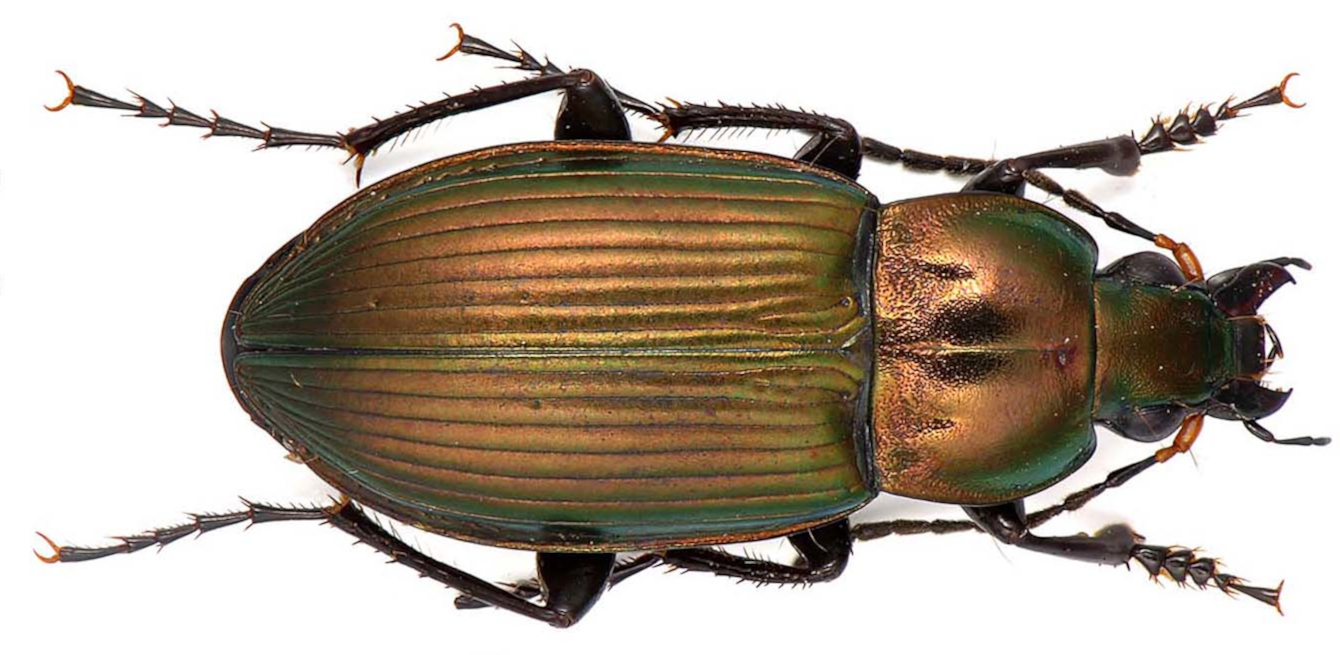
\includegraphics[width=0.60\textwidth]{images/beetle2}};
		\draw[thick,<->] (-3.2,-2.5) -- (4.7,-2.5);
		\node at (1, -2.7) {\footnotesize{12 mm}};	
	\end{tikzpicture}
	\caption{An illustration of the beetle.}
	\label{imgbeetle}
\end{figure}

In the next step, morphological landmarks were first set manually on the dorsal views of each body part of the beetles (head, pronotum, elytra, right and left mandibles). The morphology of each body part was processed and analyzed separately in order to limit variation resulting from their relative positions due to articulation. Landmarks were chosen according to the ease and the precision of their location on each specimen (Figure \ref{figdatasamples}). Replicability analyses were performed to confirm the accuracy of landmarks positioning. They were positioned on each picture with TPSDig2 software (version 2.17) (Rohlf, 2013a). In some individuals, mandibles could not be processed because they were lacking or broken. For each specific part, a set of number of landmarks has been provided, for example, \textit{$8$ landmarks for pronotum, $10$ landmarks for head, $11$ landmarks for elytra, $16$ and $18$ landmarks for left and right mandibles, respectively} (Figure \ref{figdatasamples}). In the context of this study, these manual landmarks have been used as ground truth to evaluate the output of our method.

\begin{figure}[h!]
    \centering
    \subcaptionbox{. Pronotum.}{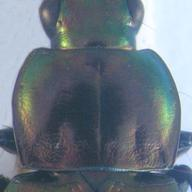
\includegraphics[width=0.19\textwidth]{./images/Prono_010}}~~
\subcaptionbox{. Head.}{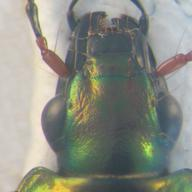
\includegraphics[width=0.19\textwidth]{./images/Tete_009}}~~
\subcaptionbox{. Elytra.}{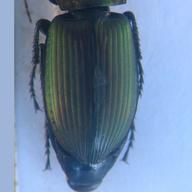
\includegraphics[width=0.19\textwidth]{./images/Elytre119}}~~
\subcaptionbox{. Left mandible.}{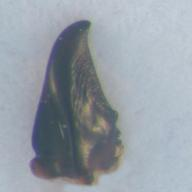
\includegraphics[width=0.19\textwidth]{./images/Mg_021}}~~
\subcaptionbox{. Right mandible.}{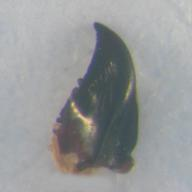
\includegraphics[width=0.19\textwidth]{./images/Md_015}}~\\
	\subcaptionbox{. Pronotum.}{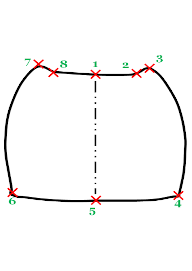
\includegraphics[width=0.19\textwidth]{./images/pronotum_mlm}}~~
\subcaptionbox{. Head.}{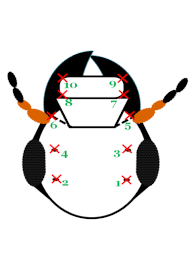
\includegraphics[width=0.19\textwidth]{./images/tete_mlm}}~~
\subcaptionbox{. Elytra.}{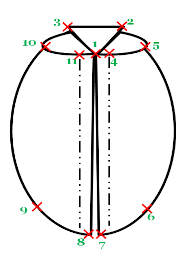
\includegraphics[width=0.19\textwidth]{./images/elytre_mlm}}~~
\subcaptionbox{. Left mandible.}{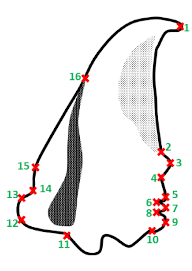
\includegraphics[width=0.19\textwidth]{./images/lmandible_mlm}}~~
\subcaptionbox{. Right mandible.}{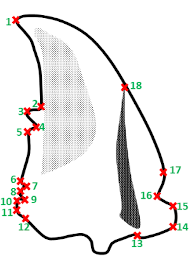
\includegraphics[width=0.19\textwidth]{./images/rmandible_mlm}}~\\
    \caption{The sample images in our dataset (top) and manual landmarks on each part defined by biologists (bottom).}
    \label{figdatasamples}
\end{figure}

The success stories \cite{krizhevsky2012imagenet, ciregan2012multi, szegedy2015going} have proved that CNN models have to be trained on a large dataset with an enormous number of data samples before using the trained model to perform on testing data. Training the model with a big dataset can help the model able to learn more different cases and to improve the learning ability of the network. Unfortunately, providing a large dataset is too costly in several domains, e.g., in biology, medicine. A solution to deal with this problem is to create the misshapen data from real data and to add them to the dataset. In our case, we have only 293 images for each part of the beetles. This number is large from the point of view of manual operations, but it is not enough to apply deep learning methods. So, we have applied data augmentation process to face this problem.

Most often in deep learning applications, dataset augmentation uses operations such as translation, rotation, or scaling, which are well-known efficient to generate new versions of existing images \cite{krizhevsky2012imagenet, shorten2019survey}. In order to select the right method for our application, we have done some tests by moving the object in the picture. In each time, we have quickly gone to the over-fitting in the training step. Consequently, we have preferred other ways to produce misshapen images by operating on the image's color channels. We have proposed two strategies to augment the number of images in our dataset.%However, these operations can be invariant in some cases \cite{shorten2019survey}.

\begin{figure}[h!]
    \centering
    \subcaptionbox{. Add a constant to each channel.}{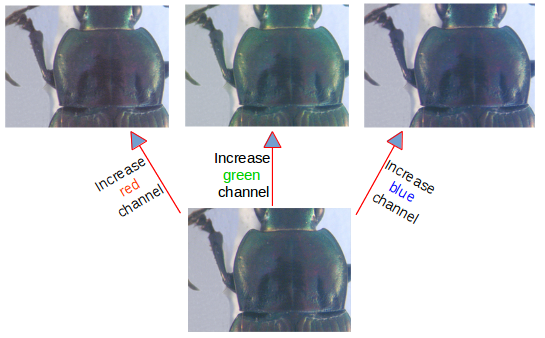
\includegraphics[width=0.49\textwidth]{./images/inc_channels}}~~
\subcaptionbox{. Split the channels of image.}{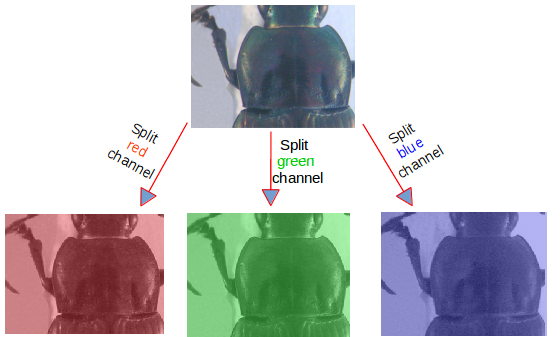
\includegraphics[width=0.49\textwidth]{./images/sp_channels}}
    \caption{The two strategies to augment the number of images in pronotum set.}
    \label{figdataauge}
\end{figure}

The first strategy was applied to change the value of each channel in the original image. According to this, a constant have been added to a channel of RGB image for each time. For example, if we add a constant $c = 10$ to the red channel from an original RGB image, we will obtain a new image with the values at red channel by greater than the red channel of original image a value of $10$. By this way, we can generate three new RGB images from a RGB image.

The second procedure was to split the channels of RGB images in order to create three gray-scale images. This work seems promising because the network model works on single-channel images. At the end, we have generated six versions from an image. In total, we have obtained $293 \times 7 = 2051$ images for each set of images. Figure \ref{figdataauge} illustrates the two described strategies.

To perform the objective, we have observed the input size of the several CNN models \cite{krizhevsky2012imagenet, ciregan2012multi, cintas2016automatic, sun2013deep} and noticed that most often their input sizes were limited to $256$ pixels. One can note that our images were released with the size of $3264 \times 2448$, as mentioned in Section \ref{subsec21}. This size is a bit heavy for training the network. Consequently, we have down-sampled our images to a new size of $256 \times 192$ to respect the ratio between width and height. Of course, coordinates of landmarks have been down-sampled to the new size of images. Practically, convergence is usually faster if the average of each input variable over the training set is close to zero \cite{lecun2012efficient}. So, the brightness of the image is normalized to $[0,1]$.% and the coordinates of the landmarks are normalized between $[-1,1]$ before giving to the network.

\subsection{Network architecture}
\label{subsec22}
Our initial trials were inspired by AlexNet architecture \cite{krizhevsky2012imagenet}. These models have been designed by combining in sequence the classical layers, e.g., convolutional (CONV), max pooling (POOL) and fully-connected (FC) layers. Unfortunately, over-fitting effects appearance very quickly. In deep learning context, it exists another type of layer, Dropout (DROP) layer, which is well-known to prevent over-fitting. After experiments, we have defined a concept of Elementary Block (EB), and utilized it as the core of our model architecture.

\begin{figure}[h!]
	\centering
	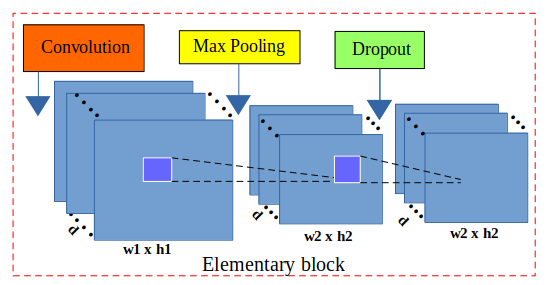
\includegraphics[width=0.5\textwidth]{images/eblock}
	\caption{The components of an elementary block}
	\label{figeblock}
\end{figure}

Figure \ref{figeblock} illustrates the order of the classes in an EB. It is defined as a sequence of a CONV layer, a maximum POOL layer, and a Dropout layer. In an Elementary Block, the convolution layer is used to extract the high-level features by applying different filters on the input. Setting POOL layer after the CONV layer towards to reduce the spatial size of the representation to decrease the number of parameters as well as to use less the computing time. The DROP layer is usually inserted between the FC layers to prevent over-fitting \cite{lecun2015deep, krizhevsky2012imagenet}, but we have included them in the extracting feature blocks to produce some kinds of image noise augmentation. The dropout layer randomly drops some connections during the training process. It makes the network thinner than the original one (fewer parameters), and training a network with dropout layer is equivalent to train a set of thinner networks. As presented in \cite{srivastava2014dropout}, DROP layer has significantly reduced over-fitting and given more considerable improvements than other regularization methods.


%As usual, the dropout layers are inserted between the FC layers to prevent the over-fitting as we have seen in the success stories \cite{lecun2015deep, krizhevsky2012imagenet}, but in our case, we have added them in the extracting features blocks (after pooling layers) to create some kinds of image noise augmentation. The objective of this work is to provide more studied cased in each training iteration. Besides, dropout layer will randomly drop some connections during the training process. It makes the network thinner than the original one (less parameters), and training a network with dropout layer is equalivalent to train a set of thinner networks. These works have significantly reduced over-fitting and given more major improvements than other regularization methods \cite{srivastava2014dropout}.
%The first model were inspired by AlexNet architecture \cite{krizhevsky2012imagenet}. It received gray-scale image with the size of $256 \times 192$ as the input. The image was analyzed by three repeated structures of a convolution (CONV) layer followed by a maximum pooling (POOL) layer. As usual, the depth of CONV layers are set to increase from the beginning to the end with a small kernel. In our model, we have chosen $32, 64, 128 $ for the depths and $ 3 \times 3, 2 \times 2, 2 \times 2 $ for the kernel's sizes of CONV layers, respectively. Using POOL layers after the CONV layers is a frequent occurrence in CNN \cite{krizhevsky2012imagenet, ciregan2012multi, cintas2016automatic}. This work towards to two advantages: reducing the spatial size of the representation to decrease the number of parameters as well as saving the computing time, and to prevent the over-fitting during the training process. In the first model, we have used the common form for a POOL layer: a filter of $2 \times 2$ with a stride of $2$ pixels. With these parameter values, the spatial size of the image will be halved after every POOL layer. In order to extract the global relationship between the features and to provide the prediction, three fully-connected (FC) layers have been added after the combination of CONV-POOL. The first FC layer takes all features from the last POOL layer as the input for computing. Then, the computed results will be passed through the activation functions to provide the outputs. The second FC layer receives the outputs of the first FC layer as the input. The process at this layer is the same than the first one. The third FC layer accepts the outputs of the second FC layer, then they will be used to compute the input. It is worth to note that we keep the linear value for the output of the third FC layer. The number of outputs at each FC layers is set to $500, 500$, and $X$, respectively. The number $X$ equals to two times the number of landmarks that we want to predict. For example, to predict $8$ landmarks on pronotum, we have set $16$ as the outputs of the last FC layer. The first model has been trained and tested on our pronotum images. Nevertheless, the obtained results have not been considered good enough to use it. The main problem comes from the appearance of over-fitting during the training process. The detail of this experiment will be discussed in Section \ref{subsec31}.

%As an attempt to remove over-fitting, we have increased the number outputs of the first two FC layers from $500$ to $1000$ with a hypothesis considering more features. However, the obtained results have not changed, the over-fitting was not suppressed.


%In order to build the third model, we have defined a concept of Elementary Block (EB). Figure \ref{figeblock} illustrates the order of the classes in an EB. It is defined as a sequence of a CONV layer, a maximum POOL layer, and a Dropout layer. As usual, the dropout layers are inserted between the FC layers to prevent the over-fitting as we have seen in the success stories \cite{lecun2015deep, krizhevsky2012imagenet}, but in our case, we have added them in the extracting features blocks (after pooling layers) to create some kinds of image noise augmentation. The objective of this work is to provide more studied cased in each training iteration. Besides, dropout layer will randomly drop some connections during the training process. It makes the network thinner than the original one (less parameters), and training a network with dropout layer is equalivalent to train a set of thinner networks. These works have significantly reduced over-fitting and given more major improvements than other regularization methods \cite{srivastava2014dropout}.

We have assembled three Elementary Blocks to create whole network architecture, called Elementary Blocks Network (EB-Net). The used parameters of layers in EBs have been set as follows: the depths of CONV layers are set to increase ($32, 64, 128$) with a small kernel ($3 \times 3$, $2 \times 2$, $2 \times 2$) from the first to the third block, respectively. The POOL layers in all three blocks have been designed with a filter of $2 \times 2$ and a stride of $2$ pixels. With these parameter values, the spatial size of the image will be halved after every block. The probabilities of the dropout layers are set increasing: $0.1, 0.2$, and $0.3$, respectively. In order to extract the global relationship between the features and to provide the prediction, three fully-connected layers have been added after the combination of EBs. The first FC layer takes all features from the last block as the input for computing. The last FC layer outputs the coordinates prediction of landmarks. The number of outputs at each FC layers is set to $1000, 1000$, and $X$, respectively. The number $X$ equals to two times the number of landmarks that we want to predict ($x, y$ coordinates). For example, to predict $8$ landmarks on pronotum, we have set $16$ as the number of outputs of the last FC layer. Additionally, a dropout layer with the probability equals to $0.5$ has been inserted between the first and the second fully-connected layers as mentioned in \cite{hinton2012improving}. Figure \ref{figebnet} resumes the EB-Net architecture.

%The used parameters of the convolution and the pooling layers in the elementary blocks have been kept in the same configuration as the second model. The probabilities of the dropout layers, which were added after the pooling layers, are set increasing: $0.1, 0.2$, and $0.3$, respectively. Following the three EBs is three fully-connected layers with a similar number of outputs as the second model.

\begin{figure}[h!]
	\centering
	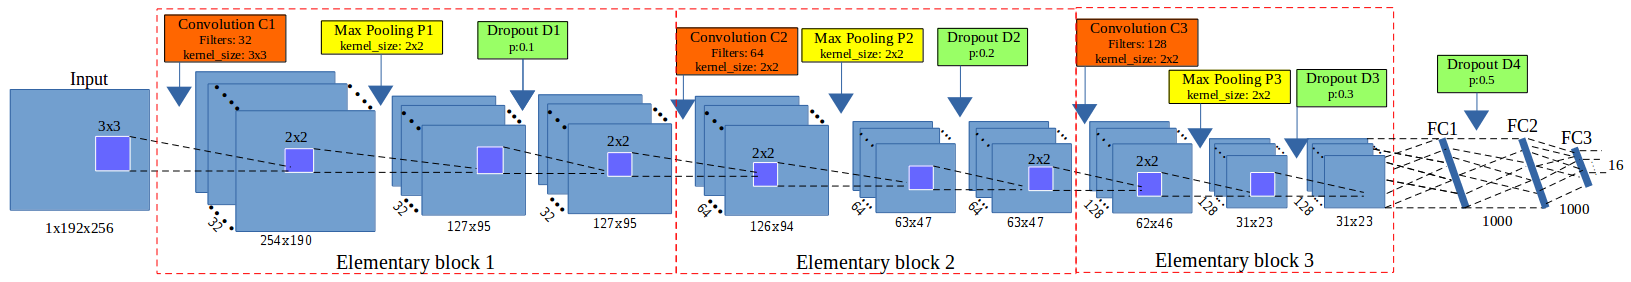
\includegraphics[width=0.99\textwidth]{images/arch_model}
	\caption{Elementary Blocks Network (EB-Net) architecture}
	\label{figebnet}
\end{figure}

In a CNN model, besides the model-specific parameters which involve the structure of the network (e.g., the number of layers or parameter values of each layer), the optimized hyper-parameters are also important variables in the designing of a CNN model. These variables are related to the training of the network model, for example, the loss function, the number of epochs, the batch size, or the initialized value of learning rate. Practically, these values are discovered through empirical observation depending on the task and the dataset. In our application, we have chosen the most common optimization algorithm, Stochastic Gradient Descent (SGD), like usual studies \cite{krizhevsky2012imagenet, cintas2016automatic}. In order to apply SGD, the two relevant parameters need to be provided: learning rate and momentum. In our application, the learning rate begins from $0.03$ and stops at $0.00001$; whereas the momentum rate is updated from $0.9$ to $0.9999$. During the training, learning rate and momentum are adjusted to fit with the number of epochs. For example, the learning rate and momentum at the first/the third epoch are $0.03/ 0.029994$ and $0.9/0.90001$, respectively. Besides, the Root Mean Square Error (RMSE) has been chosen as loss function because it is employed for regression problems where outputs represent quantitative values as the case of coordinates of landmarks. The EB-Net has been implemented by using Lasagne framework \cite{lasagne}, and trained in $5000$ epochs on Linux system by using a NVIDIA GPU (Titan X) card.

\subsection{Setting and training EB-Net}
\label{subsec23}
In order to provide the predicted landmarks for all images, we have applied cross-validation technique to select the test images, we will call a selection step is a round. For each round, we take $33$ images for testing step, the $260$ remaining images will be used to train and to validate the network model. It is worth to note that the set of $260$ images has been augmented by the strategies described in Section \ref{subsec21}, to provide $1820$ $(260 \times 7)$ images for training and validation steps. To achieve the cross-validation steps, we have to do $9$ rounds in total. 

During the training and validation step, $1820$ images are randomly divided into training and validation sets with a ratio of $60\%:40\%$. In each training step, the pair of \textit{image} and \textit{its manual landmarks} is inputted to train the network model. In the testing step, we input the image only to the trained model to predict landmarks. In our cases, the manual landmarks have been given by the biologists. So, they can be used as ground truth to train the network, as well as to evaluate the predicted ones. 

\subsection{Statistical evaluation of CNN predicted shapes}
\label{subsec24}
The quality of landmarks predicted by the network must be assessed in view of the desired usage for these predictions. It is quite frequent in geometric morphometrics to use the landmarks for subsequent procrustes regression \cite{adams_geomorph_2013} which is a method for  quantification of the relative amount of shape variation (among specimens) attributable to one or more factors in a linear model. 
Before the regression step, a generalized procrustes analysis \cite{adams_geomorph_2013} translates all specimens related landmarks to the origin, scales them to unit-centroid size, and optimally rotates them until the coordinates of corresponding points align at best. The resulting aligned coordinates represent the shape of each specimen. Afterward, the procrustes distance between specimens (i.e. sum-of-squared distance between corresponding landmarks) can be used for regression purpose \cite{goodall_procrustes_1991}. 
% One can note that using predicted landmarks instead of manual ones for procrustes regression will be a special case of Estimated Dependent Variable (EDV) models \cite{lewis_estimating_2005}. 
The crucial step that we can take to ensure the validity of using predicted landmarks for procrustes regression is a measure of shape covariation between predicted and manual landmarks \cite{rohlf_use_2000}. 
% This will be an insurance that the predicted procrustes distances are correlated between predicted and manula landmarks.
This problem is related to constructing a latent variable of shape deformation and it goes further than studying, independently, each landmark correlation between predicted versus manual. Indeed, the landmarks are not independent to each other in their relative positions between specimens because they form a shape. Hence, we are looking for covariations between predicted and manual shapes that are positive, as high as possible  and statistically significant. 

\section{Results}
\label{sec3}
\subsection{The first evaluation}
\label{subsec31}
%As mentioned in Section \ref{subsec22}, we have designed three models for our objective. In order to select the best one for our goal, we have first tested the three models on pronotum, before applying the best one on the two other parts of beetle (head and elytra).

%\begin{figure}[h!]
%    \centering
%    \subcaptionbox{. Losses of the first model.}{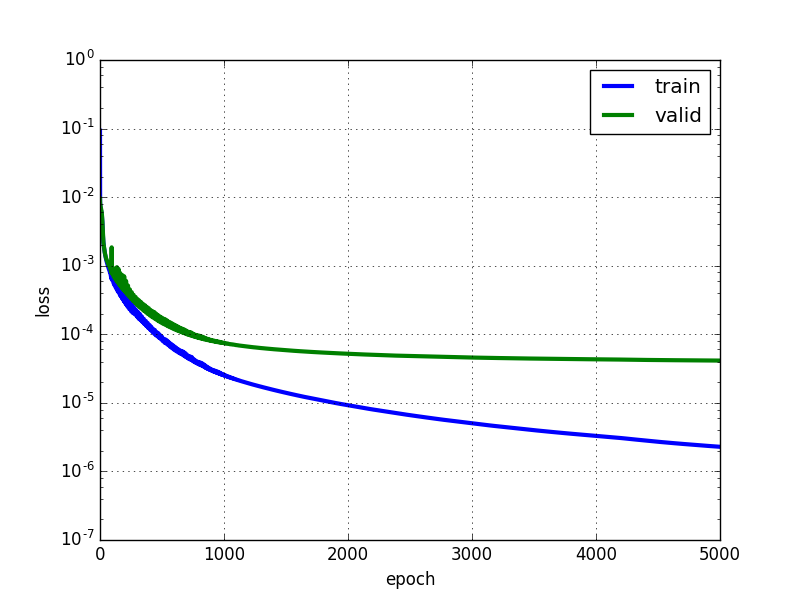
\includegraphics[width=0.43\textwidth]{./images/loss_model_1}}~~
%\subcaptionbox{. Losses of EB-Net.}{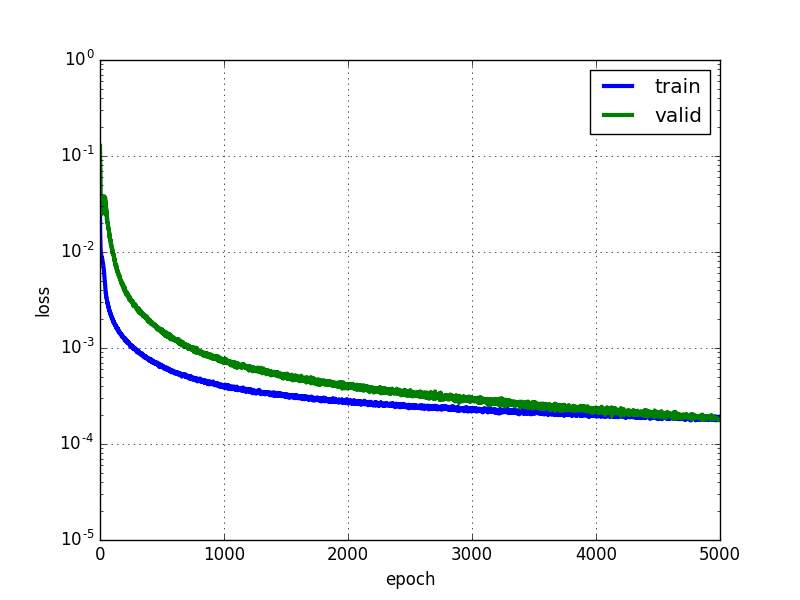
\includegraphics[width=0.43\textwidth]{./images/loss_v16}}
%    \caption{The losses of two models on pronotum images.}
%    \label{figdlosses}
%\end{figure}

%Figure \ref{figdlosses} shows the losses during the training and validation processes of two models (the first one and EB-Net) on pronotum images. The blue curves are training losses, and the green curves are validation losses. In the first model (Figure \ref{figdlosses}a), the training loss ables to decrease along with the number of epochs, but the validation loss is stable after $2000$ epochs. Clearly, the over-fitting has appeared in the fist model. In the second model, no concrete change appears in the curves even the parameters of fully-connected layers have been modified. We have also checked the losses of the second model, the result is also the same as the first one. So, we have not mentioned it in this document. On the opposite side of the first two models, the losses of EB-Net (Figure \ref{figdlosses}b) is really different. They are far from the beginning, but become more close at the end of process. One can note that the over-fitting has disappeared in this architecture. Therefore, we can assume that using elementary block works well to prevent over-fitting in our case. For these reasons, we have decided to use EB-Net for producing the landmarks.

%In order to achieve the best quality of predicted landmarks, we have tested EB-Net in two different strategies: \textit{training from scratch} and \textit{transfer learning}. The following sections describe specific results from these processes. Initially, we consider the losses during the training and validation processes. Next, we compare the coordinates of predicted landmarks and corresponding manual ones by calculating the distance between them. Then, the average distance is taken into account for each landmark position. We also display the landmarks on the image. Ultimately, the distribution of distances will be discussed in some cases of landmarks. 

EB-Net has been firstly trained and tested on the pronotum images. Figure \ref{figdlosses} shows the losses of training and validation processes of one round on pronotum images. The blue curve is the training loss, and the green curve is the validation loss. As we can notice, learning is effective and over-fitting does not appear. We can assume that EBs with the help of dropout layers have properly worked to prevent over-fitting.

\begin{figure}[h!]
    \centering
	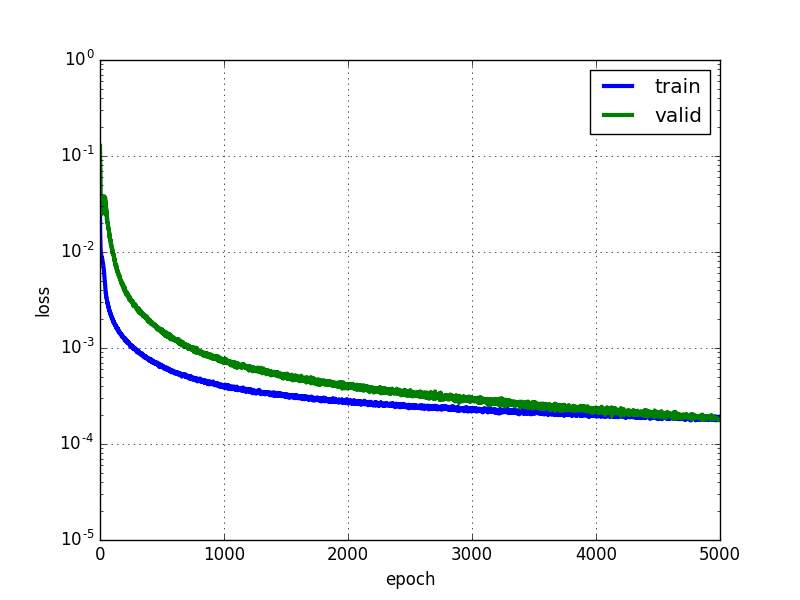
\includegraphics[width=0.45\textwidth]{./images/loss_v16}
    \caption{The losses during training EB-Net on pronotum images.}
    \label{figdlosses}
\end{figure}

Table \ref{tbltrainingloss} shows the losses of the $9$ rounds of EB-Net training on pronotum images. We can observe that although the image dataset changes through each round, the loss values remain stable and always under $3 \times 10^{-3}$. Based on the success of EB-Net on pronotum images, we have employed it on the two sets of head and elytra images with the same result qualities.

\begin{table}[h!]
	\centering
	\begin{tabular}{| c | c | c | c | c | c | c | c | c | c |}
	\hline
	Round & 1 & 2 & 3 & 4 & 5 & 6 & 7 & 8 & 9 \\ \hline
Training loss & 0.00018 & 0.00019 & 0.00019 & 0.00021 & 0.00021 & 0.00019 & 0.00018 & 0.00018 & 0.00020 \\ \hline
Validation loss & 0.00019 & 0.00021 & 0.00026 & 0.00029 & 0.00029 & 0.00018 & 0.00018 & 0.00021 & 0.00027 \\ \hline
	\end{tabular}
	\caption{The losses during the training of EB-Net on pronotum images}
	\label{tbltrainingloss}
\end{table}

The quality of performances of a CNN is mainly measured from loss, accuracy. But in this work, we also need to appreciate correctly where the estimated landmarks are positioned by the network. So, the trained model of each round has been used to predict the landmarks in images of the corresponding testing set. Then, the coordinates of outputted landmarks are evaluated by comparing with the manual ones. Figure \ref{figeb1} illustrates the landmarks on the three parts of beetles. The red/yellow points present the predicted/manual landmarks. One can note that even some predicted landmarks are close to the manual ones, we have also some predicted coordinates that are far from the expected results.

\begin{figure}[h!]
	\centering
    \subcaptionbox{. Pronotum}{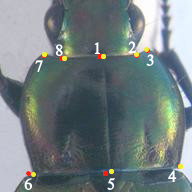
\includegraphics[width=0.30\textwidth]{images/Prono_001_2}}~~
	\subcaptionbox{. Head}{\includegraphics[width=0.30\textwidth]{images/Tete_006_2}}~~
	\subcaptionbox{. Elytra}{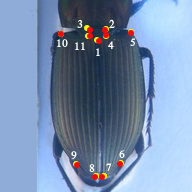
\includegraphics[width=0.30\textwidth]{images/Elytre007_2}}
    \caption{The landmarks on three parts of beetle. The red/ yellow points present the predicted/ manual landmarks.}
    \label{figeb1}
\end{figure}

In order to provide a global evaluation, the distances (in pixels) have been calculated between the manual landmarks and the corresponding predicted ones, and the average value at each position has been taken into account. Table \ref{tblavgpronotum} shows the obtained average distance for pronotum, head and elytra. With the image's size of $256 \times 192$, we can consider that an error around $1\%$ of image size ($\approx 2$ pixels) could be accepted. Unfortunately, our results exhibit the average distances from $4$ to $5$ pixels ($\approx 2\%$ of error).

\begin{table}[h!]
	\centering	
	\begin{tabular}{|c|c|c|c|c|c|c|c|c|c|c|c|}
		\hline
		\textbf{Landmark} & 1 & 2 & 3 & 4 & 5 & 6 & 7 & 8 & 9 & 10 & 11 \\ \hline
		\textbf{Pronotum} & \textcolor{green}{4.00} & 4.48 & 4.3 & 4.39 & 4.29 & \textcolor{red}{5.36} & 4.64 & 4.94 & - & - & - \\ \hline
		\textbf{Head} & \textcolor{red}{5.53} & 5.16 & 5.38 & 5.03 & 4.84 & \textcolor{green}{4.45} & 4.79 & 4.53 & 5.14 & 5.06 & - \\ \hline
		\textbf{Elytra} & \textcolor{green}{3.87} & 3.97 & 3.92 & 3.87 & 4.02 & 4.84 & 5.21 & \textcolor{red}{5.47} & 5.27 & 4.07 & 3.99 \\ \hline
	\end{tabular}
	\caption{The average distances per landmark on images of each set.}
	\label{tblavgpronotum}
\end{table}

It is worth to note that an average value could reflect two different cases: the values closed together (small dispersion) or two sets of values very far (large dispersion). In order to see in which situation we are, Figure \ref{figprodist} shows the distribution of distances between the manual and predicted landmarks for the best and the worst cases in each set of images (the green and red values in the table). Each point presents the distance between the points (landmarks) of an image. The lines (blue/red) illustrate the average distance in each case. In both of two cases (the best and the worst), the distances are most often stay in the region from 0 to the average value. Regarding these figures, it is clear that even a large number of points remain inside the range from $0$ to average value, some points are widespread between the average and $15$ or $25$ pixels. The question is it possible to correct these that. %However, it exhibits a small dispersion, some points are still far away the mean value.

\begin{figure}[h!]
    \centering
    \subcaptionbox{. The $1^{st}$ landmark (pronotum)}{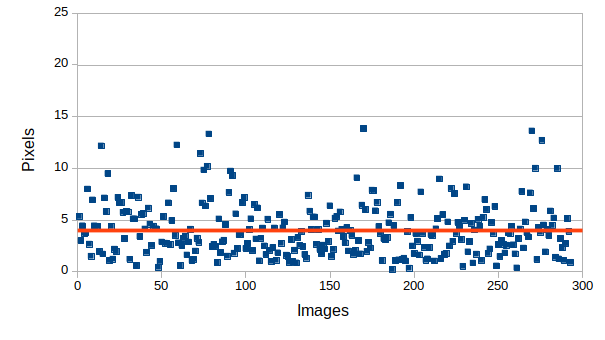
\includegraphics[width=0.44\textwidth]{./images/fs_lm1}}\hspace{0.5cm}
\subcaptionbox{. The $6^{th}$ landmark (pronotum)}{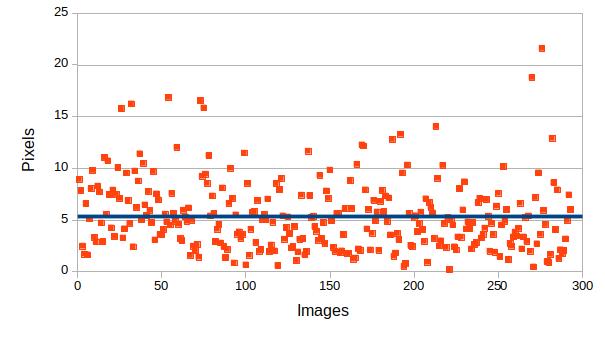
\includegraphics[width=0.44\textwidth]{./images/fs_lm6}}~\\
\subcaptionbox{. The $6^{th}$ landmark (head)}{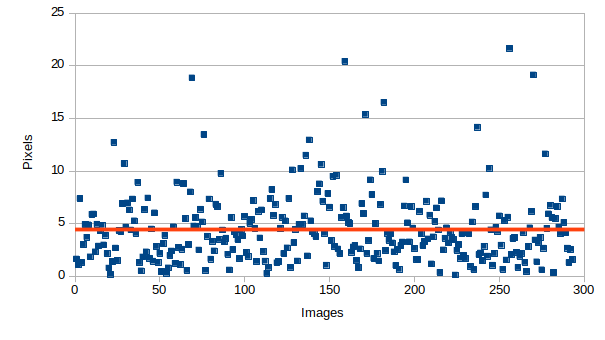
\includegraphics[width=0.44\textwidth]{./images/head6_fs}}\hspace{0.5cm}
\subcaptionbox{. The $1^{st}$ landmark (head)}{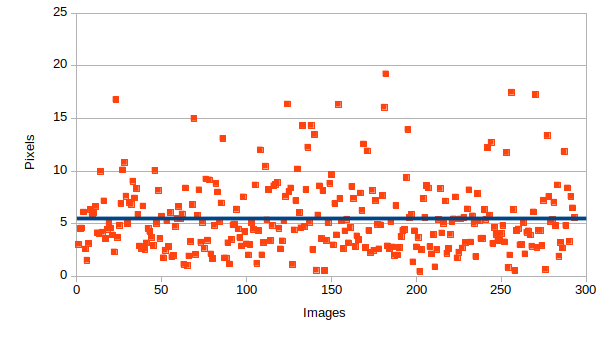
\includegraphics[width=0.44\textwidth]{./images/head1_fs}}~\\
\subcaptionbox{. The $1^{st}$ landmark (elytra)}{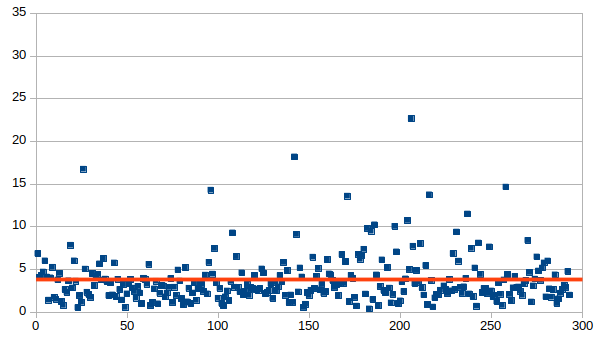
\includegraphics[width=0.44\textwidth]{./images/elytre1_fs}}\hspace{0.5cm}
\subcaptionbox{. The $8^{th}$ landmark (elytra)}{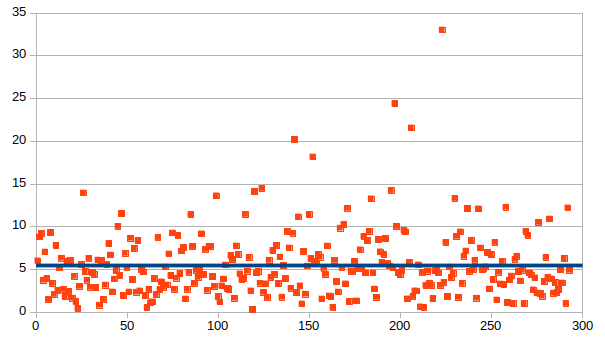
\includegraphics[width=0.44\textwidth]{./images/elytre8_fs}}
    \caption{The distribution of distances for the best and the worst cases of the three parts}
    \label{figprodist}
\end{figure}

%The EB-Net has achieved good outcomes in most cases, but it exists of several complex images in our dataset that the model has encountered a difficulty to recognize. It explains why some high distance values appeared in Figure \ref{figprodist}. The next step is to improve the predicted results.

\subsection{Transfer learning to improve performances}
Working with deep learning requires not only to design a good architecture but also to provide huge dataset to train and to test the model. Practically, this is a potential problem in some application domains as in biology. In section \ref{subsec21}, we have augmented the number of images in our dataset and used it to train EB-Net. However, our number is far away several hundred thousand images. In this case, knowledge transfer or transfer learning between tasks could be an additional solution to improve the prediction. %We describe this process in this section.

Transfer learning is a technique in deep learning to re-purpose a model which has been designed for a specific task (source task) on another related task (target task) \cite{olivas2009handbook, yosinski2014transferable}. Choosing which strategy of transfer learning to apply depending on the relationship between two tasks, as well as the size of database. Practically, transfer learning is mostly targeted on $2$ strategies:
\begin{itemize}
	\item \textbf{Use CNN as a fixed feature extractor}: Taking a CNN pre-trained on a large dataset, then removing the last fully-connected and using the rest layers of CNN as a fixed extractor for the new dataset.
	\item \textbf{Fine-tuning a CNN}: This scenario begins as the first strategy. However, it does not only replace and retrain the last layer but also fine-tunes the weights of the pre-trained model by extending the backpropagation. One can note that to reuse a pre-trained model, the parameters have to be adapted between the two tasks. These parameters could be the size of input images, the number of outputs, or the parameters of each layer.% As usual, the parameter values at each layer, e.g., padding or stride values, are selected to change their values to declare the differences between the two tasks.
\end{itemize}

In Deep Learning community, ImageNet is known as a large dataset with more than 14 million images of thousands of categories \cite{deng2009imagenet}. Notable models have employed ImageNet as training data to solve different tasks \cite{krizhevsky2012imagenet, simonyan2014very}. These pre-trained models have been widely shared in deep learning community as a source to re-use the features of ImageNet dataset. As a preliminary work, we have tested several well-known models, e.g., AlexNet \cite{krizhevsky2012imagenet}, VGG-16 \cite{simonyan2014very} that have been trained on ImageNet \cite{deng2009imagenet}. Unfortunately, the features from ImageNet seem to be not relevant for our application because the image features mainly concern the detection of global shape of the objects whereas landmarks can be considered as local features \cite{lin2016homemade}. Fortunately, searching for landmarks is explicitly defined in other applications like face recognition, or facial key-points detection. Consequently, we have decided to continue with EB-Net to improve the quality of predicted landmarks coordinates.

\subsubsection{Pre-train EB-Net on facial keypoint dataset}
In recent years, several competitions \footnote{Deepfake Detection Challenge/ Facial Keypoints Detection} have been organized for predicting facial keypoints on human face, the training datasets have been freely published. As we have mentioned, our problem has a revelant to this kind of applications. Therefore, we have decided to choose a facial keypoints dataset to pre-train EB-Net. Then, transferring the parameters values to fine-tune them for beetle's images.

The selected dataset to pre-train EB-Net has been published for a challenge\footnote{https://www.kaggle.com/c/facial-keypoints-detection} on the Kaggle website. It includes $2140$ images of human faces ($96 \times 96$ pixels). For each image, $15$ landmarks have been defined: $6$ landmarks for eyes, $4$ landmarks for eyebrows, $4$ landmarks for the mouth, and $1$ landmark for nose tip. Figure \ref{fighmface} shows $4$ examples of face images and their landmark positions in the dataset.

\begin{figure}[h!]
	\centering
	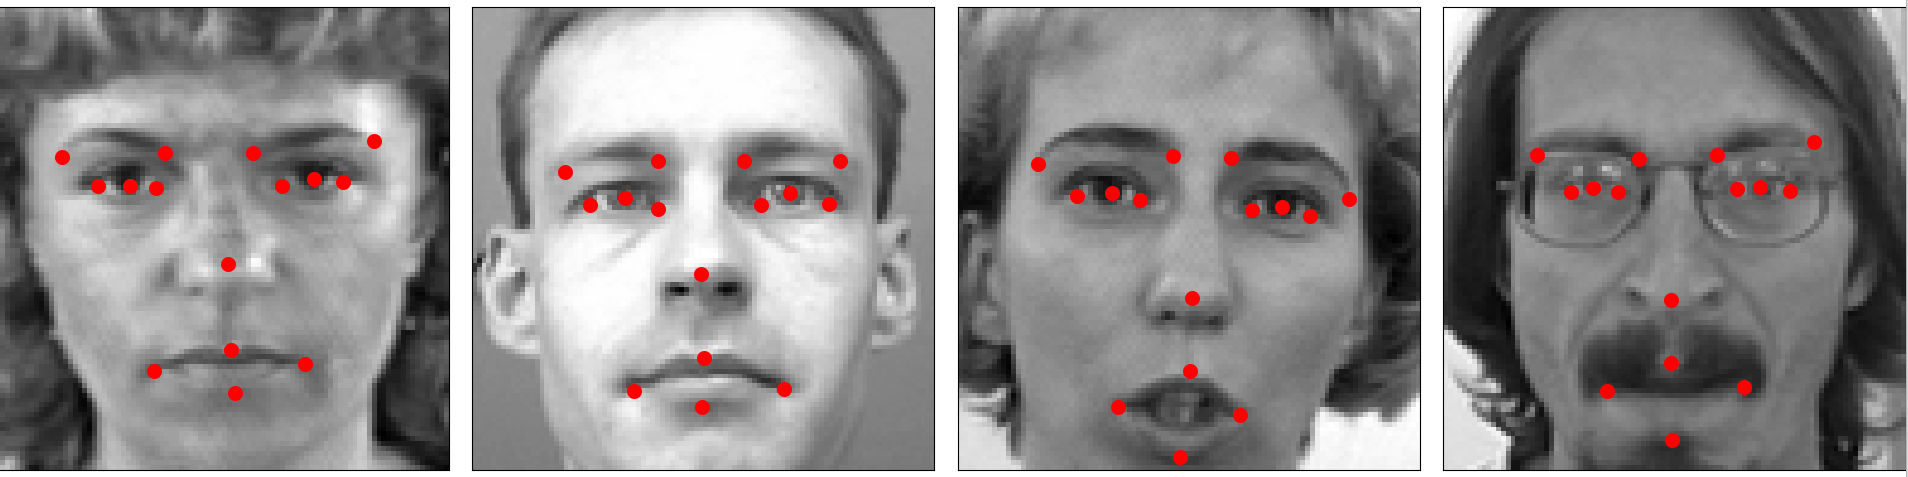
\includegraphics[width=0.80\textwidth]{images/face_dataset_2}
	\caption{The samples (face and manual landmarks) in the dataset that we used to pre-train EB-Net.}
	\label{fighmface}
\end{figure}

In order to use EB-Net on this dataset, we have adapted the parameters of the input and the output layers to match with the face images size and the landmark number. The new parameter values are $96 \times 96$ for the input size, and $30$ for the number of outputs of the last FC layer (corresponding to $15$ landmarks). For hyper-parameters, just the number of epochs have changed to reach the value of $10000$ epochs. In table \ref{tblRMSE_challenge}, we show the RMSE score and the comparison of the effectiveness between EB-Net and the three best ones that have published of the challenge.

\begin{table}[h!]
	\centering
	\begin{tabular}{ | c | c | c | c | c |}
	\hline
	%\multirow{2}{*}{Team} & Olegra & Trump & Enes & \multirow{2}{*}{EB-Net} \\ \hline
%	  & $1^{st}$ & $2^{nd}$ & $3^{rd}$ &  \\ \hline
	Team & Olegra & Trump & Enes & EB-Net \\ \hline
	RMSE score (in pixels) & 1.2824 & 1.4004 & 1.4026 & \textbf{1.497} \\ \hline
\end{tabular}	
	\caption{RMSE comparison between our score and top three of challenge.}
	\label{tblRMSE_challenge}
\end{table}

It is worth to note the three scores have been obtained by testing the models on a private set of images that are not freely available. Therefore, we have kept $100$ images from the public dataset for the testing step. Comparing with these scores, the three models present better results than us but we are very close. The RMSE score is around 1 pixel that is an acceptable error to display the landmarks on the images. Consequently, the pre-training of EB-Net is considered as correct and we have decided to re-use the pre-trained parameters values to fine-tune the model for beetle images.

\subsubsection{Fine-tuning on beetle images}
As we have mentioned, fine-tuning is a strategy of transfer learning that could boost the efficiency of a model on a target task. Technically, the weights of a CNN model can be fine-tuned by continuing the backpropagation, and it exists two ways to perform fine-tuning process: \textit{frozen} and \textit{unfrozen}.
\begin{itemize}
	\item \textbf{Frozen} scenario: the parameters of lower layers (close to the input layer) will be fixed, we fine-tune only the higher ones (close to the output layer).
	\item \textbf{Unfrozen} scenario: allows continuing to update the parameter values of all layers in the model.
\end{itemize}

In order to fine-tune EB-Net on beetle images, we have gone with unfrozen process to continue updating the parameter values. One can note that the sizes of images in the two datasets are different: the beetle images have a size of $256 \times 192$ pixels; whereas the size of facial images is $96 \times 96$ pixels. Therefore, adjustments are needed to match the two tasks.

First of all, reducing the resolution of the beetle images to $96 \times 96$ could be lead to a loss of essential information. As our images contain a background band that is easy to suppress with a pre-processing operation, we have chosen to remove a part of the background region (without any beetle's parts) instead of down-sampling our pictures. So, the new beetle images are finally set to $192 \times 192$ pixels. The EB-Net parameters will be settled to take into account the differences of the values between the pre-training and fine-tuning steps. To declare the modification, we set the stride value of the first convolutional layer to $2$ (as the usual way to do \cite{yosinski2014transferable}). 
%Moreover, removing the background pixels can limit the effect of un-useful image areas
\subsubsection{Fine-tuning results}
%To evaluate fine-tuning process, the parameters of the pre-trained model have been transferred to separately fine-tune on three sets of images: pronotum, head, and elytra. We present all the obtained results in the same way as the previous section to provide an explicit comparison. Foremost, the average distance at each landmark is provided by computing in the same way as the previous one.
%: we calculate the distances (in pixels) between predicted and corresponding manual landmarks, then these distances are used to calculate the average value for each landmark position. 
We present all the obtained results for the three beetle parts: pronotum, head and elytra, in the same way than in the previous results to provide an explicit comparison. Tables \ref{tblfn_pronotum}, \ref{tblfn_head}, \ref{tblfn_elytra} show the comparison at each position between the average distances provided by the two processes (training from scratch and fine-tuning) on pronotum, head, and elytra, respectively.  The first row presents the landmark number; \textbf{From scratch} row reminds the previously average distances when EB-Net was trained from scratch; \textbf{Fine-tune} row presents the new average distances; the last row presents the improvement percentage between the two processes. The green and red values are respectively the best and the worst values in each process. All distances are given in pixel unity. From these tables, all the average distances have decreased between $1$ and $1.5$ pixels in both of three sets of images. Clearly, the fine-tuning process has improved the prediction of landmarks, we can see the change at the best-predicted position (green ones), but it exists a group of well-predicted landmarks in each set of images, such as:

\begin{itemize}
	\item For pronotum: the $1^{st}$, $3^{rd}$, and $7^{th}$ landmark.
	\item For head: the $6^{th}$, $7^{th}$, $8^{th}$, and $10^{th}$ landmark.
	\item For elytra: the $1^{st} - 5 ^{th}$, $10^{th}$, and $11^{th}$ landmark.
\end{itemize}

At the opposite side, the worst cases remain the same positions as previously: the $6^{th}$, $1^{st}$, and $8^{th}$ landmark on pronotum, head, and elytra, respectively.

\begin{table}[h!]
	\centering
	\begin{tabular}{| c || c | c | c | c | c | c | c | c |}
		\hline
		\textbf{Landmark} & 1 & 2 & 3 & 4 & 5 & 6 & 7 & 8 \\ \hline \hline
		\textbf{From scratch} & \textcolor{green}{4.00} & 4.48 & 4.3 & 4.39 & 4.29 & \textcolor{red}{5.36} & 4.64 & 4.94 \\ \hline
		\textbf{Fine-tune} & 2.99 & 3.41 & 2.98 & 3.54 & 3.37 & \textcolor{red}{4.06} & \textcolor{green}{2.93} & 3.64 \\ \hline \hline
		\textbf{\% of impr.} & 25.25 & 24.01 & 30.56 & 19.18 & 21.55 & 24.28 & 36.85 & 26.16 \\ \hline
	\end{tabular}
	\caption{Average distances comparison on pronotum images}
	\label{tblfn_pronotum}
\end{table}

\begin{table}[h!]
	\centering
	\begin{tabular}{| c || c | c | c | c | c | c | c | c | c | c |}
		\hline
		\textbf{Landmark} & 1 & 2 & 3 & 4 & 5 & 6 & 7 & 8 & 9 & 10 \\ \hline \hline
		\textbf{From scratch} & \textcolor{red}{5.53} & 5.16 & 5.38 & 5.03 & 4.84 & \textcolor{green}{4.45} & 4.79 & 4.53 & 5.14 & 5.06 \\ \hline
		\textbf{Fine-tune} & \textcolor{red}{4.82} & 4.21 & 4.73 & 4.11 & 4.18 & 3.5 & 3.92 & \textcolor{green}{3.4} & 4.17 & 3.94 \\ \hline \hline
		\textbf{\% of impr.} & 12.83 & 18.43 & 12.15 & 18.42 & 13.69 & 21.43 & 18.29 & 24.94 & 18.88 & 22.01 \\ \hline
	\end{tabular}
	\caption{Average distances comparison on head images}
	\label{tblfn_head}
\end{table}

\begin{table}[h!]
	\centering
	\begin{tabular}{| c || c | c | c | c | c | c | c | c | c | c | c |}
		\hline
		\textbf{Landmark} & 1 & 2 & 3 & 4 & 5 & 6 & 7 & 8 & 9 & 10 & 11 \\ \hline \hline
		\textbf{From scratch} & \textcolor{green}{3.87} & 3.97 & 3.92 & 3.87 & 4.02 & 4.84 & 5.21 & \textcolor{red}{5.47} & 5.27 & 4.07 & 3.99 \\ \hline
		\textbf{Fine-tune} & 3.21 & 3.28 & \textcolor{green}{3.2} & 3.22 & 3.31 & 4.21 & 4.54 & \textcolor{red}{4.76} & 4.55 & 3.39 & 3.29 \\ \hline \hline
		\textbf{\% of impr.} & 17.04 & 17.34 & 18.36 & 16.61 & 17.66 & 13.13 & 12.82 & 12.96 & 13.69 & 16.68 & 17.54 \\ \hline
	\end{tabular}
	\caption{Average distances comparison on elytra images}
	\label{tblfn_elytra}
\end{table}

Considering on each landmark position, the improvement is different depending on the difficulty of its location. But, all cases have been improved even they are the best or the worst cases. With the help of fine-tuning, the predictions have gained from $36.85\%/ 24.94\%/ 18.36\%$ to $19.18\%/ 12.15\%/ 12.82\%$ on pronotuom, head, and elytra, respectively.

As we have mentioned before, the mean value hides different situations when deeply going to the analysis. So, we have checked again the distribution of distances. Figure \ref{figchartpfn}, \ref{figcharthfn}, \ref{figchartefn} show the distribution of distances on two samples in each set of images: pronotum, head, and elytra, respectively. In these charts, the x-axis and y-axis present the number of images and the distance (in pixel). Each point in the chart represents a distance between manual and predicted landmarks. The blue/red lines in charts present the average values. We can observe from the figures that the distance values are very different from the two processes (training from scratch and fine-tuning). The distances have been reduced with the help of fine-tuning process even they were the low or high values in the case of training from scratch. We have gained more points (in the chart) in the range from zero to the average one, and the number of extraordinary values have been decrease too. For example, in the worst case of pronotum (the $6^{th}$ landmark), we do not see any point greater than $15$ pixels with the fine-tuning process. However, it exists some difficult cases that the model could not optimize in the head or the elytra parts. These cases could be noted as the outlier values in our dataset.

\begin{figure}[h!]
    \centering
    \subcaptionbox{. $1^{st}$ landmark (from scratch) \label{}}{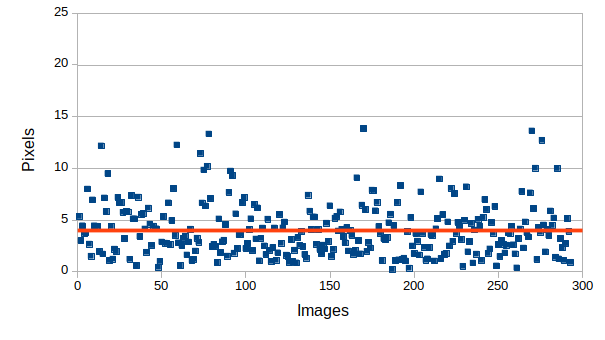
\includegraphics[width=0.47\textwidth]{./images/fs_lm1}}~~
    \subcaptionbox{. $1^{st}$ landmark (fine-tuning) \label{}}{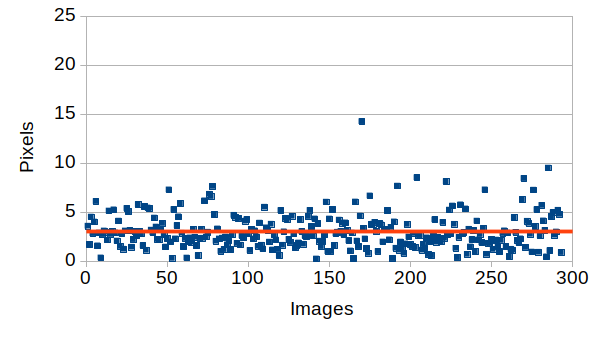
\includegraphics[width=0.47\textwidth]{./images/fn_lm1}}\\
    \subcaptionbox{. $6^{th}$ landmark (from scratch) \label{}}{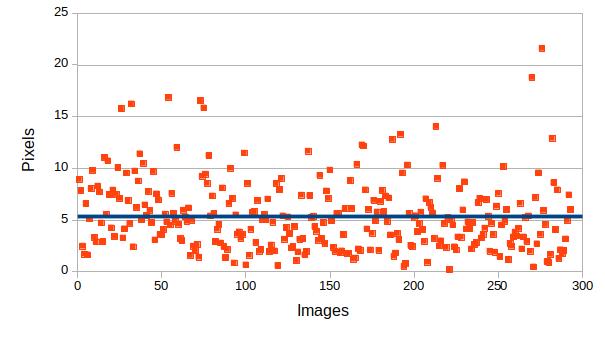
\includegraphics[width=0.47\textwidth]{./images/fs_lm6}}~~
    \subcaptionbox{. $6^{th}$ landmark (fine-tuning) \label{}}{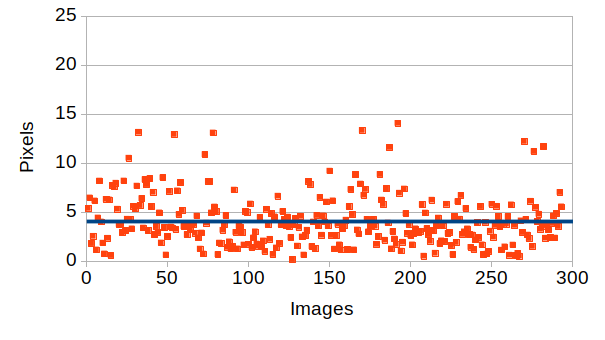
\includegraphics[width=0.47\textwidth]{./images/fn_lm6}}
    \caption{A comparison of distances distribution of the $1^{st}$ landmark and the worst case ($6^{th}$ landmark) on pronotum images. }
    \label{figchartpfn}
\end{figure}

\begin{figure}[h!]
    \centering
    \subcaptionbox{. $6^{th}$ landmark (from scratch) \label{}}{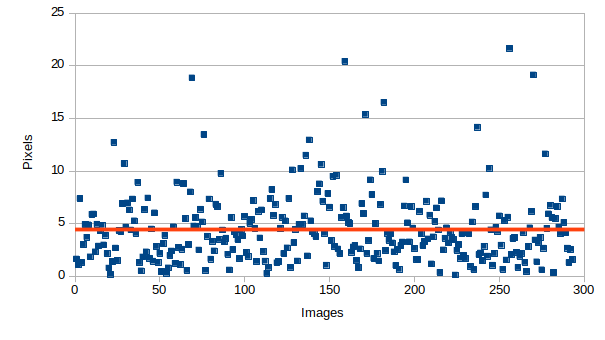
\includegraphics[width=0.45\textwidth]{./images/head6_fs}}~~
    \subcaptionbox{. $6^{th}$ landmark (fine-tuning) \label{}}{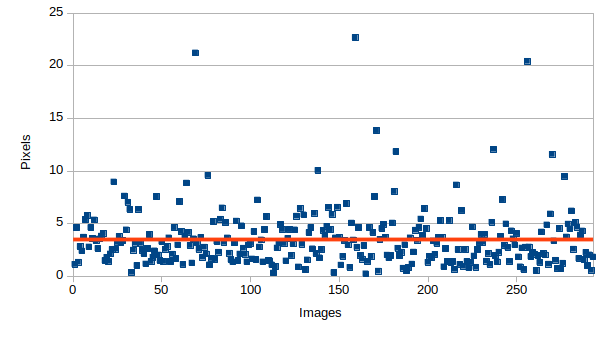
\includegraphics[width=0.45\textwidth]{./images/head6_fn}}\\
    \subcaptionbox{. $1^{st}$ landmark (from scratch) \label{}}{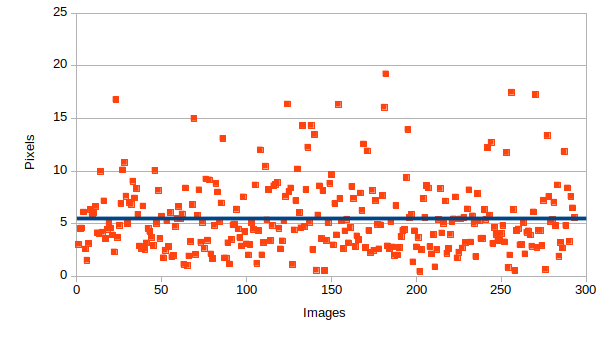
\includegraphics[width=0.45\textwidth]{./images/head1_fs}}~~
    \subcaptionbox{. $1^{st}$ landmark (fine-tuning) \label{}}{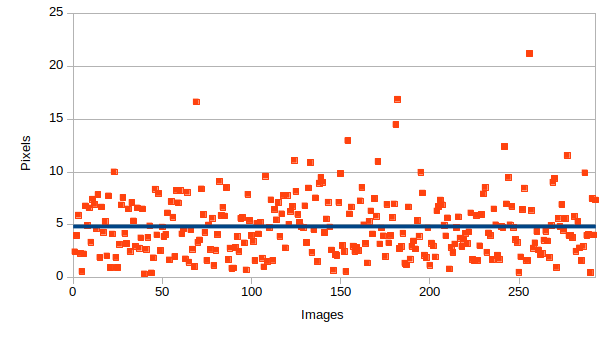
\includegraphics[width=0.45\textwidth]{./images/head1_fn}}
    \caption{The distribution of distances of all head images on $1^{st}$ landmark and $6^{th}$ landmark. }
    \label{figcharthfn}
\end{figure}

\begin{figure}[h!]
    \centering
    \subcaptionbox{. $1^{st}$ landmark (from scratch) \label{}}{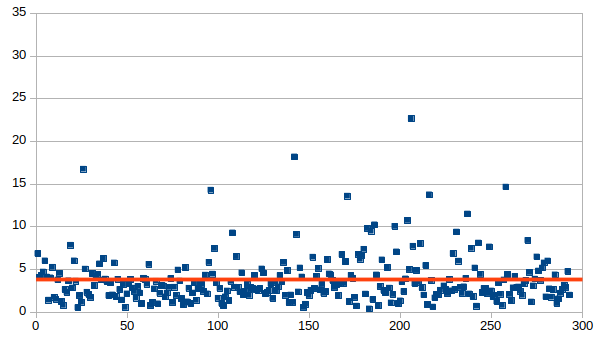
\includegraphics[width=0.45\textwidth]{./images/elytre1_fs}}~~
    \subcaptionbox{. $1^{st}$ landmark (fine-tuning) \label{}}{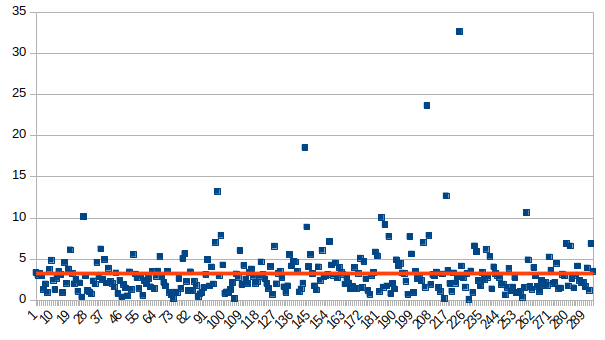
\includegraphics[width=0.45\textwidth]{./images/elytre1_fn}}\\
    \subcaptionbox{. $8^{th}$ landmark (from scratch) \label{}}{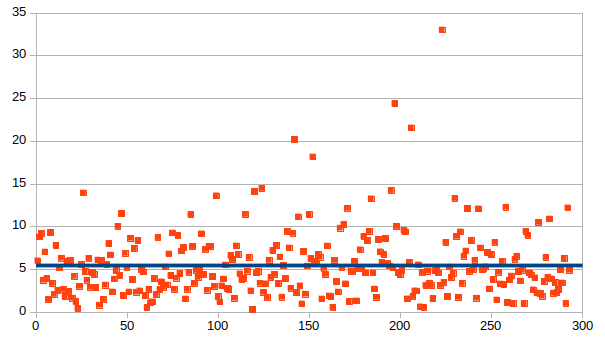
\includegraphics[width=0.45\textwidth]{./images/elytre8_fs}}~~
    \subcaptionbox{. $8^{th}$ landmark (fine-tuning) \label{}}{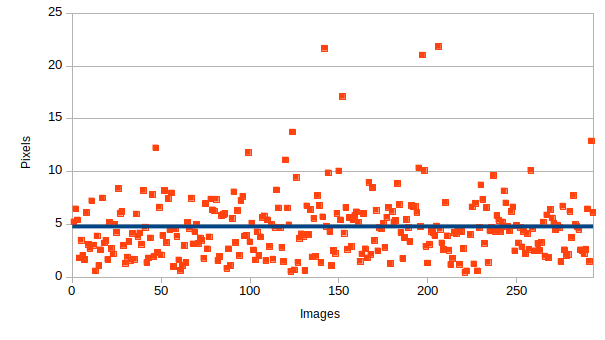
\includegraphics[width=0.45\textwidth]{./images/elytre8_fn}}
    \caption{The distribution of distances of all elytra images on $1^{st}$ landmark and $8^{th}$ landmark.}
    \label{figchartefn}
\end{figure}

To illustrate the results, Figure \ref{figpdl} shows both predicted (in red) and manual (in yellow) landmarks on three random images from the three sets of images. Clearly, the predictions have been improved, they are more close to the manual ones. For example, we have obtained $7$ well-predicted landmarks on the head images.

\begin{figure}[h!]
    \centering
    \subcaptionbox{. Pronotum \label{}}{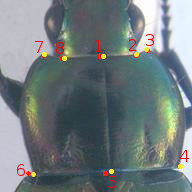
\includegraphics[width=0.3\textwidth]{./images/Prono_001}}
    \subcaptionbox{. Head \label{}}{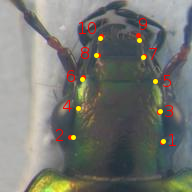
\includegraphics[width=0.3\textwidth]{./images/Tete_005}}
    \subcaptionbox{. Elytra \label{}}{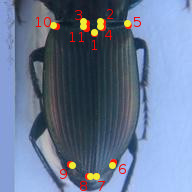
\includegraphics[width=0.3\textwidth]{./images/Elytre004}}
    \caption{The location of predicted/manual landmarks in one case of each part.\\The red/yellow points represent the predicted/manual landmarks.}
    \label{figpdl}
\end{figure}

%\pagebreak
\subsubsection{Results on mandibles}
As mentioned in previous work \cite{le2017maelab}, the mandible images have been analyzed with the help of a pipeline based on the segmentation step. We have evaluated the performances of EB-Net on this dataset. It is worth to note that the fine-tuning process has been applied for this experiment in the same way than the other parts: pre-training EB-Net with the facial key-points dataset and transferring the parameter values to fine-tune on mandibles.

To achieve the comparison, the obtained values in \cite{le2017maelab} have been re-computed to match the new size of the images by scaling these errors (distances) with the same ratio that we have used to down-sample images. Then, the average value has been computed for each landmark’s position. Figure \ref{figchartavgCompare} shows the comparison of average distance at each landmark position between the obtained results of the two methods (deep learning and image processing methods). The red curves illustrate the average distances which have been obtained from image processing technique while the blue curves present the results of fine-tuning process. 

\begin{figure}[h!]
    \centering
	\subcaptionbox{. Right mandible \label{figchartavgComparemd}}{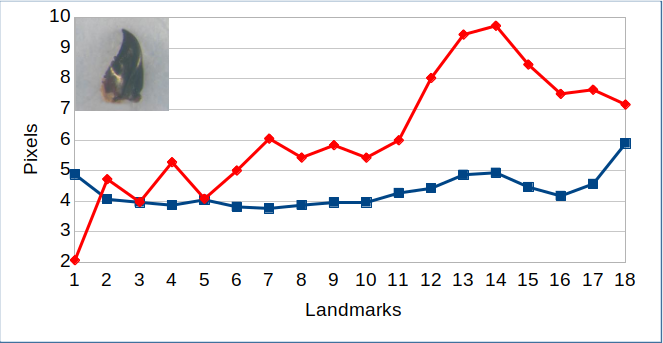
\includegraphics[width=0.49\textwidth]{./images/md_avg_comparison}}~~    
    \subcaptionbox{. Left mandible \label{figchartavgComparemg}}{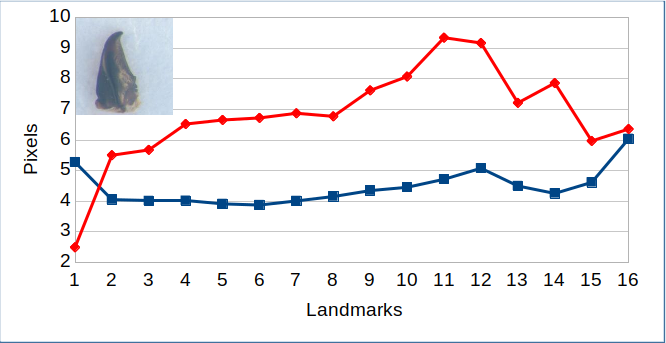
\includegraphics[width=0.49\textwidth]{./images/mg_avg_comparison}}    
    \caption{These charts show the average distance on each landmark of all mandibles images.\\ The red, blue lines present the results from image processing and fine-tuning process, respectively.}
    \label{figchartavgCompare}
\end{figure}

For the right mandible (Figure \ref{figchartavgComparemd}), EB-Net has got better results than the image processing pipeline for all landmarks (except the first one). One can notice that the first position represent the tip of the shape, and it is easy to detect after a segmentation step. EB-Net works without segmentation, it is why the result for this point is similar to the other ones. Moreover, it is clear that the results of EB-Net exhibit of less variation than the previous method. For the left mandible (Figure \ref{figchartavgComparemg}), the pipeline has provided the worst results than for the right one. The hypothesis has been given that the size of this part varies more than the right one. On the opposite side, we can observe that EB-Net has produced results similar to the right one.

To summarize, the average value at each landmark position is better than the previous ones in both two cases: left and right mandibles, with the help of the fine-tuning process. The predictions are more stable and significantly improved: it has reduced the range between the highest and the lowest values in both of two sets, for example, from $6.85/ 7.66$ pixels to $2.17/ 2.13$ pixels for the left and right mandibles, respectively.

\subsubsection{Predicted shapes : comparing 'from-scratch' to fine-tuning}

We have measured shape covariations between predicted landmarks and manual ones \cite{rohlf_use_2000}, assessing the performance of fine-tuned and `from scratch' networks (described previously) on each anatomical parts. The shape covariation is expressed as a correlation coefficient and an associated p-value.

\begin{table}[h!]
	\centering
	\begin{tabular}{| c || c | c | c | c |}
		\hline
		  & \multicolumn{2}{ c |}{From scratch}  & \multicolumn{2}{ c |}{Fine-tune} \\ \cline{2-5}
		  & cor & p-value & cor. & p-v. \\ \hline
		\textbf{Pronotum} & 0.4118 & 0.001 & 0.7424 & 0.001 \\ \hline 
		\textbf{Head} & 0.5145 & 0.001 & 0.7337 & 0.001 \\ \hline 
		\textbf{Elytra} & 0.2513 & 0.407 & 0.3025 & 0.069 \\ \hline 
		\textbf{Left mandible} & 0.2666 & 0.173 & 0.3112 & 0.057 \\ \hline 
		\textbf{Right mandible} & 0.3071 & 0.239 & 0.4597 & 0.002 \\ \hline 
	\end{tabular}
	\caption{Shape covariation between predicted and manual landmarks : shape covariation as a correlation (cor.) and an associated p-values (p-v.) }
	\label{tblfsft_comparing}
\end{table}

We can see from table \ref{tblfsft_comparing} that shape correlations varies between $0.2513$ and $0.7424$ and that $5$ out of $10$ of them are statistically significant (i.e. p-value $< 0.05$). For all the anatomical parts, the fine-tuning improved the shape correlations. For all the correlations with  p-values $> 0.05$, the fine tuning improved at the same time the correlation strength and the statistical significance. Best results are obtained for fine-tuned networks predicting pronotum's and head's  landmarks with high significant correlations, $0.7224$ and $0.7337$ respectively. Right mandible predictions by fine tuned network is also of interest with a mild correlation ($0.4597$) but still significant (p-value $= 0.002$). We end up with a majority ($\frac{3}{5}$) of anatomical parts were the predicted landmarks are good candidate for replacing manual ones in any procrustes regressions.

\section{Discussion and perspectives}

In this article, we have presented a convolutional neural network, EB-Net, for automatically predict the landmarks on entomological images. It is based on three times the repetitions of a generic block followed by fully connected layers. The block consists of a convolutional layer, a max-pooling layer, and a dropout layer. In the first step, the EB-Net has been separately trained on each part of the beetles. In order to improve the results, the fine-tuning process has been added by pre-training EB-Net on a facial key-points dataset before transferring the parameter values to fine-tune on each set of images.

The results have been evaluated by calculating the distance between manual landmarks and predicted ones. These results have shown that using CNN to predict the landmarks on biological images leads to satisfying results without need for the complex pre or post processing steps on the studied objects. These predictions are statistically significant enough to replace manual landmarks in procrustes regression studies, which are fairly common in morphometric studies e.g. two classic methodological papers on the subject\cite{goodall_procrustes_1991,collyer_method_2015} have a combined $299$ direct citations and we can assume that most citations are indirect.

This work has addressed a complex task in computational biology: automatic landmark digitalization. The interest in this topic is not new, but the relevant algorithms and computational power have only been available fairly recently \cite{palaniswamy_automatic_2010,cintas_automatic_2017,vandaele_landmark_2018,dai_locating_2019}. Even so  most methods are seldom used by biologist and even so by entomologist. 
Maybe it is because the software tools are too complex and the necessary datasets not always available (e.g. too few training images and related manual landmarks).
We show here that a neural network with a relevant architecture can provide a high quality of results in only a few methodological steps. We took care of constructing this network using standard software tools to ease any technological transfer. Also, our model, EB-Net, can easily work with a limited number of images and improve its prediction results by fine-tuning the parameter values obtained from pre-training on another dataset.

One can note that the elementary block that we used to build EB-Net, is generic so it's easy to adjust the suitable number of blocks for ones applications depending on the computing resources, as well as the expected results. For example, we have tried to add a new elementary block to EB-Net. The experiments have shown that the results have been slightly improved, but we have spent more resources and computing times to reach this improvement. The average distances have been improved by $0.5$ pixels. However, this change was statistically insignificant (data not shown). Consequently, we need to note that it exists a balance between the depth of the model, the accuracy of outputs and the cost to compute.
This elementary block approach is not, formally, a  neural architecture search \cite{elsken_neural_2019} i.e. a method for automating the design of a CNN,  but it is an easy to implement practical solution.

In this application, we focused on a carabid species which is linked to studies in agroecology and conservation ecology. But EB-Net has the potential to be applied to other insects and invertebrates as well.
So in the future, we plan to test our model on more  
datasets that are linked to other ecological fields most notably invasive species and quarantine species (e.g. nematods). All the implementations, EB-Net model and EB-Net parameters, are available freely \footnote{\url{ https://github.com/linhlevandlu/cnnBeetles}}. It is possible to reuse EB-Net parameters for another landmark setting application and to apply transfer learning. We plan also to export EB-Net architecture to other application domains in biomedicsl imaging most notably MRI images analysis. 

%\section*{References}

\bibliography{includes/references}

\end{document}











%This work has addressed a complex task in digital biology: automatized landmarks setting. We show that a neural network with a relevant architecture can provide an outstanding quality of results with reducing the number of steps. Our model, EB-Net, is one of them. The obtained results have pointed out that EB-Net easy to work on a limited number of images, and simply to improve results by fine-tuning the parameter values obtained from pre-training on another dataset.

%This work has addressed a complex task in digital biology: automatized landmarks setting. We show that a neural network with a relevant architecture can provide a high quality of results with reducing the number of steps. If training a network remains a costly operation, utilizing it is not time-consuming nor spends so much memory.
%Our model, EB-Net, has been built from elementary blocks and used to provide the landmarks on beetle images by applying two scenarios: training from scratch and fine-tuning process. The results have shown that our network architecture has worked effectively for predicting the landmarks. One can note that the model is independent of the segmentation step, it has analyzed the raw image through a sequence of elementary blocks before providing the location of landmarks. Moreover, the predictions have figured out that we have obtained better results with the help of the fine-tuning process. This point out that EB-Net is easy to work on a limited number of images, and simply to improve results by fine-tuning the parameter values obtained from pre-training on another dataset. It also shows the obtained results are more stable than the pipeline of image processing techniques.

One can note that the elementary block that we used to build EB-Net, is a generic one. It is easy to compose to build a network or even to remove a block from the model if the results are not satisfying. The users can select the suitable number of blocks for their applications depending on the computing resources, as well as the expected results. For example, we have tried to add a new elementary block to EB-Net. The experiments have shown that the results have been improved but not enough to justify the supplementary cost in resources or computing time.

All the implementations of EB-Net model and the pre-trained parameter values are available freely on the Github website \footnote{https://github.com/linhlevandlu/CNN\_Beetles\_Landmarks}. It is possible to download and to re-use them for another landmark setting application by training from scratch or applying transfer learning process.

% Remarkably, the fine-tuning has a great improvement at the positions located at parts that are hard to extract the contours. More, these results are stable on every landmark position. with image processing techniques, some first landmarks (from $1^{st}$ to $6^{th}$) have been well-predicted, which illustrated by small average values in the chart. However, these values begin to increase from the $7^{th}$ landmark. The reason is that the first group of events is mainly concentrated on the tip of the mandible where we can obtain the precise segmentation, while others are on the base where we can meet some difficulties to get the segment contours. For the fine-tuning process, the obtained values are more stable. Although some first values can be approximate or larger (from $2^{nd}$ to $7^{th}$ positions), other ones are better than the previous results (after $7^{th}$ position). Remarkably, the fine-tuning has a great improvement at the positions located at parts that are hard to extract the contours. More, these results are stable on every landmark position. 

\section{Conclusion}
In this article, we have presented a convolutional neural network, EB-Net, for automatic detection of landmarks on biological species. It is based on three times repeated of a generic block followed by the connected layers. The block consists of a convolutional layer, a max pooling layer, and a dropout layer. In the first step, the EB-Net has been separately trained on each part of beetles. In order to improve the results, the fine-tuning process has been added by pre-training EB-Net on a facial keypoints dataset from Kaggle before transfering the parameter values to fine-tune on each set of images.

The results have been evaluated by calculating the distance between manual landmarks and predicted ones. These results have shown that using CNN to predict the landmarks on biological images leads to satisfying results without need for segmentation step on the studied objects. These results have been valided by biologists in order to replace the manual task by the automatic one.

In future, we plan to test our model on different datasets owned by the INRA team, and to export EB-Net architecture for applying to other application domains studied in our team such as MRI images analysis, pose identification.

%For each set of images, different selections of data have been used to train, to validate, and to test the model. After training with the manual landmarks given by the biologist, the network is able to predict the landmarks on the set of unseen images. The results from the test set have been evaluated by calculating the distance between manual landmarks and corresponding predicted-landmarks. The average of distance errors on each landmark has been also considered. Using the convolutional network to predict the landmarks on biological images is promising good results in the case that the image can not be segmentation. The quality of prediction allows using automatic landmarking to replace manual landmarks in some aspects. In our case, the training dataset is limited. As a result, the accuracy of the network is acceptable. However, when we expect more about the accuracy of predicted landmarks (coordinates of predicted landmarks), the result of this work is still needed to improve (for example using a larger training dataset).

%In the second strategy to improve the results, EB-Net has been pre-trained on a facial keypoints dataset, then the parameter values have been transferred to fine-tune on each set of images. The predicted coordinates have been also evaluated by calculating the distance to manual ones. The results have shown that we have obtained the improvement in all cases of landmarks with the help of fine-tuning process. Therefore, future research in landmarking identification appears as an improved of the worth exploring.

%\subsection{Evalution metrics for further predicted landmarks usage}

%TODO \\

















%In this work, we have proposed a CNN network architecture for predicting landmarks in beetle images. The model is based on the concept of elementary block including a CONV layer, a Max POOL layer, and a Dropout layer. 

%With beetle mandibles images, the object is easy to segment and we have succeeded to determine the landmarks automatically. In opposite, the pronotum images are difficult to segment. Methods which not suppose to be based on segmentation are necessary. 




%For the right mandible (Figure \ref{figchartavgComparemd}), some first landmarks (from the $1^{st}$ to the $6^{th}$) have been well-predicted by the pipeline of image processing techniques. They are illustrated by the small average values in the chart (from $2.07$ pixels to $9.73$ pixels). However, these values begin increasing from the $7^{th}$ landmark and peak at the $14^{th}$ position. The reason is the first group of landmarks is mainly concentrated on the tip of the mandible where we can obtain the precise segmentation, while the others are on the base and we can encounter some difficulties to get the segment contours. For the fine-tuning process, all distances are better than the previous results (except the first one). The obtained values are more stable, and the variants between the results are not so large as in the previous one.

%For the left mandible (Figure \ref{figchartavgComparemg}), we obtain the similar situation than the right one. The obtained average values are more stable and better than the results coming from previous method (except the first one). One can note that the left mandibles are more difficult to process than the right ones by using image processing technique as discussed in \cite{le2017maelab}. The proof is that the values of the precise predictions (between $1^{st}$ and $8^{th}$) in the left mandibles are higher than the right ones. 

\section{Discussion}
In this work, we have proposed the elementary block as the based to build the CNN for predicting landmarks. It is worth to note that our block is a generic one. It is easy to add it, easy to test the model, even to remove a block from the model if the results are not satisfying. The users can choose suitable blocks for their applications. Choosing the number of blocks depends on the computing resources, as well as the expected results. For example, we have tried to add a new elementary block to EB-Net. The experiments have shown that the results have been improved, but we have spent more resources and computing times to reach this improvement. The average distances have been improved $0.5$ pixels. However, this change is insignificant if we show it on the images. Consequently, we need to note that it exists a balance between the depth of the model, the accuracy of outputs and the cost to compute.

\textbf{TODO}: on biological part.

As mentioned in section \ref{subsec21}, the mandible images have been taken after dissection, whereas the images of other parts have been captured before this process. In \cite{le2017maelab}, we have proposed a pipeline based on the segmentation step and applied to mandible images. The results have shown the pipeline has worked efficiently to provide the automatic landmarks on mandibles, but it could not be applied on the three parts of beetle: pronotum, head and elytra. It is why we have turned to utilize the CNN model for these three parts. In this experiment, we would like checking that if CNN work well to predict the landmark on mandible images. We have applied the fine-tuning process to mandible images in the same way than other parts. Then, we compare the obtained results between the two processes (fine-tuning and pipeline in \cite{le2017maelab}). 

In the five sets of beetle images, the mandibles are considered as easy to extract by using the image processing algorithms. In \cite{le2017maelab}, we have proposed a pipeline to estimate the landmarks in mandible images. In order to evaluate the effectivement of deep learning method and to compare with the obtained results from \cite{le2017maelab}, we have applied the fine-tuning process on mandible images in the same way as we have done on other parts. 

 In hyper-parameters side, we have increased the number of epochs to $10000$ but kept the same for other values as training from scratch. As the first step, we take into account the RMSE score to evaluate and to compare the effectiveness of EB-Net with other published scores in the challenge.



 The appearance of POOL layer after the CONV layer is a frequent occurrence in CNN \cite{krizhevsky2012imagenet, ciregan2012multi, cintas2016automatic}. This work towards to two advantages: reducing the spatial size of the representation to decrease the number of parameters as well as saving the computing time, and to prevent the over-fitting during the training process. The dropout layer is usually inserted between the FC layers to prevent over-fitting as we have seen in the success stories \cite{lecun2015deep, krizhevsky2012imagenet}. But in our case, we have included them in the extracting features blocks (after pooling layers) to create some kinds of image noise augmentation. The objective of this work is to provide more studied cased in each training iteration. 




 Then, the computed results will be passed through the activation functions to provide the outputs. The second FC layer receives the outputs of the first FC layer as the input. The operations at this layer are the same than the first one. The third FC layer accepts the outputs of the second FC layer, then they will be used to compute the input.





In the content of this study, we work on pronotum part of beetle. The provided dataset contains 293 images, each image with 8 landmarks provided by biologists. The dataset was split into a training set with 260 images (training and validation) and a testing set of 33 images. During the training, the network learned the information through a pair of \textit{(image, landmarks)} in training set. At the testing phase, the image without landmarks was given to the trained network and the predicted landmarks will be given at the output. Fig. \ref{figpronotum} shows an example of pronotum image with its manual landmarks.

\begin{figure}[h!]
	\centerline{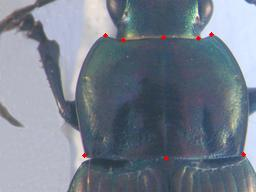
\includegraphics[scale=0.8]{images/pronotum}}
	\caption{An example of pronotum with manual landmarks}
	\label{figpronotum}
\end{figure}

In some succeed networks \cite{krizhevsky2012imagenet}\cite{sun2013deep}\cite{cintas2016automatic}, the maximum size of the inputs is not over 256 pixels. In our case, the resolution of the image is large, it becomes a difficulty for the network. During training and testing, the images are down-sampling to the new resolution of $256 \times 192$. Certainly, the landmark coordinates of the image are also scaled to suit their new resolution. 

The proposed network has a large number of learnable parameters. In addition, the size of the dataset is limited, this means that overfitting will occur during the training process. Therefore, we need to enlarge the size of the dataset. In image processing, we usually apply transform procedure (i.e rotate, translate) to generate a new image but in fact, when we compute the value of the pixels, it does not change while CNN computes the values of the pixels.Therefore, we have applied two other procedures to increase the number of images in the dataset. To address this problem, we have applied two procedures to enlarge the size of the dataset.

The first procedure was applied to change the value of each channel in the original image. According to this, a constant is added to a channel of RGB image and for each time, we just change the value of one of three channels. For example, from an original RGB image, if we add a constant $c = 10$ to the red channel, we will obtain a new image with the values at red channel by greater than the red channel of original image a value of 10. By this way, we can generate three new RGB images from a RGB image.

The second procedure is splitting the channels of RGB images. It means that we separate the channels of RGB into three gray-scale images. This work seems promising because the network works on single-channel images. At the end, we can generate six versions from an image, the total number of images used to train and validate is $260 \times 7 = 1820$ images (six versions and original image). The number of images that used for training and validation is splitted randomly by a ratio (training: $80\%$, validation: $20\%$) that has been set during the network setup.